\chapter{Analyse de la distribution d'un marqueur de l'attention au sein d'une population d'enfants TDAH}

\section*{Introduction}
Le \gls{tbr} a été massivement étudié chez les enfants \gls{tdah}. Diminuer le \gls{tbr} est par ailleurs un protocole d'entrainement de \gls{nfb} couramment utilisé 
pour traiter le \gls{tdah} chez les enfants \citep{Arnold2014, Deilami2016, Gevensleben2009, VanDongen2013}. Cependant, ce protocole ne serait peut-être pas adapté à tous les enfants \gls{tdah} si 
on se base sur le phénotype de leur \gls{eeg}. En effet, il a été avancé qu'il existerait un groupe d'enfants \gls{tdah} présentant un \gls{tbr} élevé 
\citep{Zhang2017, Clarke2011}, ainsi ces enfants bénéficieraient peut-être davantage d'un protocole diminuant leur \gls{tbr} que les autres. 

Quelques études ont proposé de personnaliser le protocole d'entrainement par \gls{nfb} \citep{Bazanova2018, Escolano2014}, mais trop peu pour en déterminer
l'impact sur l'efficacité du \gls{nfb} par la \gls{saob}. L'analyse présentée dans ce chapitre n'a pas pour but d'évaluer directement l'efficacité de la 
personnalisation des protocoles de \gls{nfb} mais sa pertinence. Pour ce faire, la distribution des valeurs de \gls{tbr} chez les enfants \gls{tdah} est 
étudiée à l'aide de différentes méthodes de partitionnement pour déterminer combien de groupes d'enfants \gls{tdah} existent en se basant seulement sur les 
valeurs de \gls{tbr}. 

\section{Population étudiée}

Les signaus \gls{eeg} utilisés dans cette analyse proviennent de trois bases de données différentes :
\begin{itemize}
\item NEWROFEED (NCT02778360, Mensia Technologies, France, ClinicalTrials.gov, \citet{Bioulac2019}),
\item \gls{cmi-mipdb} \citep{Langer2017, Langer2017b},
\item \gls{cmi-hbn} \citep{Alexander2017, Alexander2017b}.
\end{itemize}
Pour chacune de ces bases de données, un consentement éclairé écrit a été obtenu de tous les participants ou de leurs responsables légaux. Tous les enregistrements
ont été effectués dans un environnement contrôlé avec les yeux ouverts (\gls{eo} en anglais) et au repos (c'est à dire que le sujet n'effectue aucune tâche) 
pendant une minute sous la supervision d'un clinicien ou d'un chercheur. 

La description de l'ensemble des données est disponible dans la Table~\ref{Table:tbr_datasets_description}.

\begin{table}[h!]
  \centering
  \caption{Informations sur les données utilisées. Les critères d'inclusion pour chaque base de données sont listés, ainsi que le nombre de sujets satisfaisant
	chaque critère entre parenthèses. Le nombre total de sujets inclus par base de données est précisé à la dernère ligne.}
  \fontsize{9}{11}\selectfont
\begin{tabular}{ ccccc }
\toprule
Base de données & NEWROFEED & CMI-MIPDB & \multicolumn{2}{ c }{CMI-HBN} \\
\midrule
\shortstack{ Description \\ de la population } & \shortstack{ - 7-13 ans \\ - Diagnostiqué \gls{tdah} \\ - Enregistré avec \\ l'appareil
                                               \\ Mensia Koala\textregistered : \\ 8 électrodes \\ du système 10-20 } 
																							 & \shortstack{ - 6-44 ans \\ - Avec et sans \\ diagnostic \\ - Enregistré avec \\ le système
                                               \gls{eeg} \\ Geodesic Hydrocel : \\ 128 électrodes } 
																							 & \multicolumn{2}{ c }{ \shortstack{ - 5-21 ans \\ - Avec et sans \\ diagnostic \\ - Enregistré avec \\ le système
                                               \gls{eeg} \\ Geodesic Hydrocel : \\ 128 électrodes } }
																							\\
\midrule
Nombre de sujets & \shortstack{ 122 (données disponibles \\ au 09/2017 pour les \\ analyses de contrôle \\ de la qualité avant \\ la fin de l'étude \\ en 12/2017) } 
                 & 126 
								 & \multicolumn{2}{ c }{ 881 }
								\\
\midrule
\shortstack{ Critères d'inclusion \\ additionnels} & \shortstack{ 1. Age/diagnostic \\ précisés (122) \\ 2. \textbf{Diagnostic} \\ \textbf{ \gls{tdah} } (122) \\ 3. \gls{eeg} d'une \\ min \gls{eo} 
                 au repos \\ disponible et \\ possible à \\ analyser (122) } 
                 & \shortstack{ 1. Age/diagnostic \\ précisés (126) \\ 2. \textbf{Diagnostic :} \\ \textbf{ \gls{tdah} } (12) \\ 3. \gls{eeg} d'une \\ min \gls{eo} 
                 au repos \\ disponible et \\ possible à \\ analyser (10) } 
								 & \shortstack{ 1. Age/diagnostic \\ précisés (447) \\ 2. \textbf{Diagnostic :} \\ \textbf{ \gls{tdah} } (237) \\ 3. \gls{eeg} d'une \\ min \gls{eo} 
                 au repos \\ disponible et \\ possible à \\ analyser (231) } 
								 & \shortstack{ 1. Age/diagnostic \\ précisés (447) \\ 2. \textbf{Diagnostic :} \\ \textbf{ Aucun }  (76) \\ 3. \gls{eeg} d'une \\ min \gls{eo}  
                 au repos \\disponible et \\ possible à \\ analyser (74) } 
								\\
\midrule
\shortstack{ Nombre de \\ sujets inclus} & 122 & 10 & 231 & 74 \\
\bottomrule
\end{tabular}
  \label{Table:tbr_datasets_description}
\end{table}

\subsection{Données NEWROFEED}

Une partie des données utilisées dans cette analyse provient de l'étude NEWROFEED (NCT02778360, Mensia Technologies, France, ClinicalTrials.gov, \citet{Bioulac2019})
qui avait pour but d'évaluer l'efficacité du \gls{nfb} à la maison versus celle du méthylphenidate sur une population d'enfants \gls{tdah}.
Au moment où le travail décrit dans ce chapitre a été mené, NEWROFEED était en cours donc 
seulement une partie des données était disponible. Ainsi, 122 enregistrements \gls{eeg} d'enfants diagnostiqués \gls{tdah} d'après les critères du DSM-IV \citep{DSM-4} 
ont été analysés. L'\gls{eeg} a été enregistré avec l'appareil Mensia Koala équipé de 8 électrodes \gls{agcl} individuellement blindées, positionnées sur le scalp suivant
le système international 10-20 : Fpz, F3, Fz, F4, C3, Cz, C4, Pz. La fréquence d'échantillonnage était de 512Hz. Les impédances devaient être
inférieures à $40$k$\Omega$ et le niveau de contamination électromagnétique devait rester inférieur à 1/3 de l'énergie totale du signal. 

Pour participer à l'étude NEWROFEED, les sujets devaient remplir les critères suivants :
\begin{enumerate}
\item être des enfants ou adolescents (fille ou garçon) entre 7 et 13 ans,
\item avoir un diagnostic \gls{tdah} positif avec Kiddie-SADS \citep{Kaufman1997},
\item avoir un score sur l'ADHD RS IV supérieur à 6 pour l'inattention, avec ou sans hyperactivité \citep{Pappas2006}.
\end{enumerate}

De plus, les enfants correspondant à un de ces critères ont été exclus :
\begin{itemize}
\item être \gls{tdah} avec le sous-type hyperactif/impulsif mais sans la composante inattention,
\item avoir un trouble psychiatrique sevère et/ou incontrôlable autre que le \gls{tdah} diagnostiqué avec Kiddie-SADS tel que par 
exemple l'autisme ou la schizophrénie,
\item avoir un trouble comorbide nécessitant des médicaments psychoactifs autres que ceux prescrits pour le \gls{tdah},
\item avoir un QI < 80 d'après les trois sous-tests du WASI ou du WISC \citep{Wechsler1999}.
\end{itemize}

Seule la première évaluation de l'\gls{eeg} enregistrée pour chaque patient avant le début du traitement par \gls{nfb} est utilisée pour cette analyse. 
L'étude NEWROFEED a été menée dans 12 centres cliniques dans 5 pays européens (France, Espagne, Allemagne, Belgique et Suisse).

\subsection{Données CMI-MIPDB}
Au moment de l'analyse, l'intégralité de la base \gls{cmi-mipdb} compte 126 participants à la fois avec et sans diagnostic clinique \citep{Langer2017, Langer2017b}.
Les participants ont été recrutés au Child Mind Medical Practice et dans la région de la ville de New-York. Chaque sujet a été questionné pendant 10 minutes
au téléphone ou en personne par un chercheur expérimenté pour évaluer son éligibilité grâce à :
\begin{itemize}
\item l'historique de ses troubles psychiatriques, incluant les traitements en cours et précédents,
\item l'historique de ses troubles neurologiques et/ou épilepsie.
\end{itemize}

L'enregistrement de l'\gls{eeg} est prévu si aucune contre indication n'est trouvée. 

De tous les patients présents dans la base \gls{cmi-mipdb}, seulement ceux satisfaisant les critères suivants ont été inclus dans l'analyse présentée dans ce chapitre :
\begin{enumerate}
\item être diagnostiqué\gls{tdah},
\item posséder un \gls{eeg} au repos disponible au format ".raw",
\item avoir son âge précisé.
\end{enumerate}

L'\gls{eeg} a été enregistré avec un système \gls{eeg} Geodesic Hydrocel à une fréquence d'échantillonnage de 500Hz et un filtre passe-bande entre 0.1 et 100Hz. 
L'électrode de référence est Cz, localisée au vertex de la tête. Le tour de tête de chaque participant est mesuré pour que le bonnet utilisé lors de l'enregistrement 
soit à la bonne taille. L'impédance des électrodes est gardée inférieure à $40$k$\Omega$ : elle est vérifiée toutes les 30 minutes ainsi qu'avant chaque enregitrement.

\subsection{Données CMI-HBN}
La base de données \gls{cmi-hbn} est composée de 881 sujets, avec ou sans diagnostic \citep{Alexander2017, Alexander2017b}. Les familles recoivent 150\$ pour leur participation 
et les sujets se voient de plus offrir les rapports de consultation et les avis sur les sessions d'\gls{eeg}.

Seuls les sujets remplissant les critères suivants ont été inclus dans notre analyse :
\begin{enumerate}
\item être diagnostiqué \gls{tdah} selon le KSADS-COMP \citep{Kaufman1997},
\item posséder un \gls{eeg} au repos disponible au format matlab ".mat",
\item avoir son âge précisé.
\end{enumerate}

Des 881 sujets disponibles, 231 (âgés entre 5 et 21 ans) satisfont ces critères et sont inclus dans notre analyse.

La base de données \gls{cmi-hbn} contient également des sujets sains qui vont être utilisés en tant qu'\textit{a priori} (\textit{priors} en anglais) pour le
modèle bayesien décrit en \ref{clustering}. Pour être inclus dans cette analyse en tant que \textit{priors}, les sujets ne doivent avoir aucun diagnostic 
et doivent remplir les critères 2. et 3. cités précédemment. Au final, 74 sujets entre 5 et 21 ans sont sélectionnés. 

\subsection{Pré-traitement et homogénéisation des bases de données} \label{pré-traitement TBR}
Les \gls{eeg} des différentes bases de données sont pré-traités de façon à être comparables, notamment au niveau du placement des électrodes.
En ce qui concerne le traitement des artefacts et l'extraction du \gls{tbr}, les étapes sont les mêmes quelle que soit la base de données. 
Les pré-traitements ainsi que les analyses des signaux \gls{eeg} qui suivent sont effectués à l'aide du logiciel NeuroRT (v3, Mensia Technologies, 
Paris, France).

\subsubsection{Base de données NEWROFEED}
Le seul pré-traitement que nécessitent les signaux de la base de données NEWROFEED est un filtrage temporel : 
\begin{itemize}
\item un filtre Butterworth passe-haut d'ordre 1 à 0.5Hz afin d'enlever la composante continue (\textit{DC component} en anglais),
\item un filtre Butterworth coupe-bande d'ordre 3 de 47 à 53Hz afin d'enlever l'artefact causé par les lignes électriques.
\end{itemize}

\subsubsection{Bases de données CMI}

Le pré-traitement des bases de données \gls{cmi-mipdb} et \gls{cmi-hbn} demande plus d'étapes : filtrage temporel, suppression et 
interpolation des canaux bruités et/ou déconnectés, et une interpolation spatiale afin de passer d'un espace à 128 électrodes \gls{egi},
à l'espace de 8 électrodes placées selon le système 10-20 utilisé dans la base de données NEWROFEED.

Tout d'abord, les \gls{eeg} obtenus au repos sont séparés en deux fichiers : l'un pour les enregistrements les yeux fermés, 
l'autre pour les enregistrements \gls{eo}, seul ce dernier va être analysé. Ensuite, les mêmes filtres temporels vont être appliqués
que pour les données NEWROFEED, à l'exception du filtre coupe bande dont les bornes sont modifiées pour intercepter les artefacts 
causés par les lignes électriques américaines (57-63Hz).

Dans le cas d'enregistrements d'\gls{eeg} avec une haute résolution spatiale comme ici avec les données CMI, 
il est courant qu'au moins un canal se déconnecte ponctuellement causant aussi bien des artefacts de large amplitude que des signaux plats. 
Une strategie est ici mise en place pour détecter de façon fiable puis interpoler ces électrodes déconnectées : la variance de chaque canal 
\gls{eeg} est calculée sur une fenêtre glissante de 10 secondes puis est ensuite convertie en deux z-scores grâce à :
\begin{enumerate}
\item la distribution instantanée des variances pour les 127 autres canaux (z-score spatial),
\item la distribution cumulative des variances pour le canal d'intérêt (z-score temporel).
\end{enumerate}
Si le z-score temporel n'est pas compris entre -5 et 5, le signal est détecté comme étant un artefact et est interpolé à partir des canaux voisins.
Si le z-score spatial n'est pas compris entre -2 et 2, soit le signal a une trop grande variance (autrement dit il est bruité), soit une trop faible
variance (autrement dit l'électrode doit être déconnectée et n'energistre rien) : dans les deux cas il est interpolé.

Les données sont re-référéncées sur l'électrode de la mastoïde gauche (électrode 57 de l'\gls{egi}-128) pour correspondre au référencement de la base
de données NEWROFEED. Les signaux \gls{eeg} des 128 électrodes de l'espace \gls{egi} sont ensuite spatialement reconstruits dans l'espace à 8 électrodes 
dans le système international 10-20 en projetant les coordonnées sur une sphère unitaire.


\section{Theta-Beta ratio : un marqueur de l'attention}

\subsection{Définition du Theta-Beta ratio}
La littérature indique qu'il existerait différents groupes de patients \gls{tdah} identifiés à l'aide de leur profil \gls{eeg}, comme l'augmentation
de la puisssance dans la bande theta et/ou la diminution de la puissance dans la bande beta \citep{Clarke2011, Loo2018}. Ces différences de puissances dans ces 
bandes de fréquence peuvent être quantifiées en calculant la ratio de la puissance dans la bande theta et de la puissance dans la bande beta : le 
\gls{tbr} \citep{Arns2013}. 

De nombreuses études ont été menées pour analyser la pertinence d'utilser le \gls{tbr} comme biomarqueur pour diagnostiquer le \gls{tdah}. En effet, certains auteurs suggèrent qu'un \gls{tbr}
élevé peut aider à confirmer les diagnostics du \gls{tdah} \citep{NebaHealth, Saad2018, FDA}. Cependant, les études récentes ont échoué à repliquer les résultats
montrant une différence entre les valeurs de \gls{tbr} des patients \gls{tdah} et celles des patients sains, remettant en question son utilisation comme outil 
diagnostic \citep{Zhang2017, Arns2013, Clarke2001}. A la place, ces études trouvent qu'environ 35\% des sujets \gls{tdah} présenteraient un \gls{tbr} élevé : ce
résultat pourrait être utilisé pour identifier de meilleurs répondeurs à une intervention donnée. 

La diminution du \gls{tbr} fait partie des protocoles le plus couramment utilisé en \gls{nfb} appliqué aux enfants \gls{tdah} \citep{Arns2014}. 
On peut soutenir que l'efficacité de ce traitement pourrait être augmentée en affectant chaque patient à l'entraînement qui correspond le mieux à son phénotype \gls{eeg}. 
Par exemple, les sujets présentant un haut \gls{tbr} suivraient un protocole de \gls{nfb} où il est demandé de diminuer le \gls{tbr}. Cette répartition a été proposée lors 
de l'essai clinique NEWROFEED, pour lequel un seuil de répartition a dû être choisi. Un essai clinique randomisé et en double aveugle proposé par \citet{Kerson2013} 
prévoyait d'utiliser un seuil \gls{tbr} de 5 mais cette valeur a été modifiée et fixée à 4.5 (NCT02251743, Arnold, Ohio State University, ClinicalTrials.gov), valeur également
utilisée dans NEWROFEED. Choisir correctement la valeur de seuil est crucial car cette valeur détermine quel protocole de \gls{nfb} le patient va suivre. 

Le caractère arbitraire des valeurs de seuil basées sur le \gls{tbr} appelle à une validation précise de l'existence d'un 
sous-groupe de patients \gls{tdah} présentant un \gls{tbr} élevé et du le seuil à partir duquel les valeurs de \gls{tbr} sont considérées comme élevées.  
 
\subsection{Extraction du Theta-Beta ratio}
L'extraction du \gls{tbr} des \gls{eeg} pré-traités après \ref{pré-traitement TBR} comprend plusieurs étapes :
\begin{enumerate}
\item le rejet des artefacts en utilisant la géométrie Riemannienne,
\item l'extraction de l'\gls{iapf},
\item le calcul du \gls{tbr}.
\end{enumerate}

\subsubsection{Rejet des artefacts}
Tout d'abord, les données artefactées sont exclues en utilisant le \gls{rpf} \citep{Barthelemy2019}. Les données \gls{eeg} sont ségmentées (durée de 2 secondes avec 
un chevauchement toutes les 0.125s) et la matrice de covariance de chaque segment est calculée pour un sous-ensemble de canaux. Ensuite, la \gls{rpf} rejette les 
segments dont la matrice de covariance se retouve à l'extérieur d'une région d'acceptabilité définie grâce à une référence d'\gls{eeg} propres. 

\subsubsection{Extraction de l'\textit{individualized Alpha Peak Frequency}}
Ensuite, l'\gls{iapf} est calculée en déterminant la fréquence à laquelle le pic de puissance est observé dans la bande alpha définie entre 7 et 13Hz. Si aucun pic n'est observé,
l'\gls{iapf} est obtenue grâce à l'estimation de Klimesch basée sur l'âge du sujet \citep{Klimesch1999}. L'\gls{iapf} est calculée sur l'\gls{eeg} mesuré à l'électrode Pz au repos
et les yeux ouverts. 

L'\gls{iapf} permet de définir des bandes de fréquence personnalisées pour chaque sujet : theta = [\gls{iapf} - 5Hz ; \gls{iapf} - 1Hz], beta = [\gls{iapf} + 3Hz ; \gls{iapf} + 12Hz].
Cette étape a pour but d'adapter précisément l'entrainement aux jeunes cerveaux qui se développent très vite. En effet, dans le cas des enfants, il serait possible de considérer 
des basses fréquences de la bande alpha comme appartenant à la bande theta, ce qui fausserait l'entrainement par \gls{nfb} car la modulation de mauvaises fréquences 
seraient récompensée. Cette méthode mène évidemment à des résultats différents d'avec des bandes de fréquence aux bornes fixes \citep{Arns2008, Vollebregt2015} et a été 
l'objet de plusieurs études \citep{Kaiser2001, Bazanova2006, Vollebregt2015} dont les résultats montrent que cette personnalisation pourrait améliorer l'efficacité du protocole
\gls{tbr} pour le traitement du \gls{tdah}.

\subsubsection{Calcul du Theta-Beta ratio}
La dernière étape consiste à calculer le \gls{tbr} : il est défini comme le ratio de la puissance dans la bande de fréquences theta et de la bande de fréquences beta obtenues 
grâce à l'\gls{iapf}. Une moyenne mobile de la puissance du signal $\bar{P}$ est estimée par la méthode de Welch \citep{Welch1967} sur 32 segments, de 2 secondes chacun, avec un 
chevauchement toutes les 1/16 de seconde :
\begin{equation}
\label{eq:tbr_power_computation}
P_{c,b} = \norm{ x_{c,b} }_{F}^2,
\end{equation}
\begin{equation}
\label{eq:tbr_average_power_computation}
\bar{P}_{c,b} = \frac{1}{I} \sum_{i=1}^{I} (P_{c,b})_{i},
\end{equation}
où $x_{c,b}$ correspond à un segment du signal \gls{eeg} sur le canal $c$ après un filtre passe-bande sur la fréquence $b$, $\norm{.}_{F}$ est la norme de Frobenius et $I$ 
le nombre de segments. La puissance dans les bandes theta ($\theta$) et beta ($\beta$) est calculée avec les équations Eq.~(\ref{eq:tbr_power_computation}) et Eq.~(\ref{eq:tbr_average_power_computation}),
puis ces deux puissances sont divisées entre elles :

\begin{equation}
\label{eq:tbr_tbr_computation}
\text{TBR} = \frac{\bar{P}_{c,\theta}}{\bar{P}_{c,\beta}},
\end{equation}
conduisant à un ratio instantané de valeurs de puissances qui représente une implémentation en temps réel du \gls{tbr}.

La distribution de l'ensemble des $\bar{P}_{c,b}$ n'étant pas normale, la mediane obtenue à Fz et Cz est utilisée pour représenter le \gls{tbr} sur l'ensemble 
de l'enregistrement. Le maximum sur ces deux électrodes est retenu, il sera enfin normalisé pour les analyses suivantes en un \gls{srntbr} :

\begin{equation}
\label{eq:tbr_srntbr_computation}
\text{srnTBR} = \sqrt{ \text{max}(\frac{\bar{P}_{Fz,\theta}}{\bar{P}_{Fz,\beta} } ; \frac{\bar{P}_{Cz,\theta}}{\bar{P}_{Cz,\beta}} ) }.
\end{equation}

\subsection{Méthodes de partitionnement de la distribution des Theta-beta ratios} \label{clustering}

Afin de déterminer s'il existe un groupe d'enfants \gls{tdah} présentant un \gls{tbr} élevé, trois méthodes de partitionnement (\textit{clustering} en anglais) 
sont mises en place : une qui se base sur les distributions (\gls{bgmm}), une sur les distances (la méthode de Ward) et une autre sur 
les densités (\gls{dbscan}). Les analyses statistiques sont effectuées avec la bibliothèque Python Scikit Learn (V0.18.1, \citet{Pedregosa2011}).

\subsubsection{Partitionnement basé sur les distributions : Bayesian Gaussian Mixture Model} 
Un \textit{mixture model} est un modèle probabiliste qui permet d'identifier la présence de sous-populations dans une population.
La distribution des \glspl{srntbr} est ainsi tracée et ajustée par un \gls{bgmm} \citep{Attias2000, Blei2006} puis par 
un \gls{gmm} pour comparaison. Un \textit{Gaussian Mixture Model} est un modèle qui suppose que toutes les observations proviennent d'un mélange 
d'un nombre fini de distributions gaussiennes aux paramètres inconnus. 
Le \gls{bgmm}, à la différence du \gls{gmm}, utilise des \textit{a priori} sur la distribution des données pour 
assigner des probabilités \textit{a posteriori} à chaque \textit{Gaussian Mixture} distribution. Un grand nombre de \glspl{tbr} 
extraits de sujets sains de la base de données \gls{cmi-hbn} est disponible, ces valeurs sont donc utilisées pour estimer les \textit{a priori} du \gls{bgmm}. 
Lorsque les observations sont ajustées par un \gls{bgmm} ou un \gls{gmm}, un modèle gaussien constitué d'un nombre prédéfini de courbes gaussiennes est 
créé pour modéliser les données. Ici, les valeurs de \gls{srntbr} sont approximées par un \gls{bgmm} avec un nombre de composantes allant de 1 à 3. 
Il en va de même pour l'algorithme du \gls{gmm}.

Afin de déterminer le nombre de composantes qui décrit le mieux la distribution des \gls{srntbr}, la significativité de la différence entre chaque 
modèle est testée grâce à un test $\chi^2$ sur la déviance \citep{James2013}. La déviance est une mesure de la qualité de l'ajustement (\textit{goodness-of-fit} 
en anglais) d'un modèle statistique et est définie comme suit :
\begin{equation}
\label{eq:tbr_deviance}
\text{D} = -2(log(L(\beta_{0})) - log(L(\beta_{\alpha}))),
\end{equation}
où $log(L(\beta_{0}))$ est la \textit{log likelihood} du modèle nul et $log(L(\beta_{\alpha}))$ est la \textit{log likelihood} du modèle alternatif. 
La \textit{log likelihood} a pour rôle de donner une idée sur la capacité des données à résumer les paramètres de la distribution de probabilités. 
La multiplication par -2 est une étape nécessaire pour convertir la \textit{log likelihood} en une distribution \textit{chi-square} qui permet 
l'utilisation d'un test $\chi^2$ pour tester la significativité statistique. Le seuil de significativité est fixé à $\alpha = 0.01$.

\subsubsection{Partitionnement basé sur les distances : méthode de Ward}
La méthode de Ward fait partie des algorithmes de partitionnement hiérarchique \citep{Ward1963}. 
Cet algorithme est un type d'\textit{agglomerative clustering} qui, de façon récursive, fusionne une paire de groupes 
en minimisant la variance de ces \textit{clusters} jusqu'à obtenir un grand \textit{cluster} comprenant toutes les données.

Le nombre de clusters estimé ici par Ward varie de 1 à 3 pour comparer les résultats obtenus à ceux du \gls{bgmm}. Les \textit{clusters}
identifiés par la méthode Ward sont notamment représentés sur un dendrogramme où les traits verticaux correspondent à la distance de Ward entre 
deux \textit{clusters} : plus ces traits sont grands, plus les clusters son différents

\subsubsection{Partitionnement basé sur les densités : DBSCAN}
\gls{dbscan} est un algorithme de partitionnement de données qui s'appuie sur la densité des \textit{clusters} estimés \citep{Ester1996}. 
Deux paramètres sont nécessaires pour permettre à l'algorithme de partitionner la donnée : la distance $\epsilon$ et le nombre minimum de points 
$MinPts$ devant se trouver dans un rayon $\epsilon$ pour que ces points forment un \textit{cluster}. 
Le choix du $MinPts$ peut se faire grâce une méthode heuristique :
\begin{equation}
\label{eq:tbr_dbscan}
MinPts = ln(\text{n}),
\end{equation}
avec n le nombre total de points à être partitionnés.

Une méthode pour déterminer la valeur $\epsilon$ optimale est de tracer le graphique des \textit{k-distance} obtenu par la méthode des k plus proches voisins 
(\gls{knn} en anglais) non supervisée en prenant $k = MinPts$ \citep{James2013, Goldberger2005}. Le principe de cette méthode
est de trouver un nombre prédéfini d'observations, noté k, les plus proches en distance d'un nouveau point et de prédire la classe de ce dernier. 
Le grahique des distances k (\textit{k-distance plot} en anglais) représente les distances de chaque observation à un des k points classées par ordre décroissant. 
Ainsi, étant donné que les points bruités sont censés avoir une \textit{k-distance} bien plus élevée que celle des autres points, on peut 
s'attendre à observer un coude sur ce tracé : l'ordonnée de ce point correspond à $\epsilon$.

Le \textit{silhouette coefficient} est utilisé pour rendre compte de la qualité du partitionnement : -1 est la pire valeur, 1 la meilleure et 0
correspond à des \textit{clusters} qui se superposent.

\subsection{Identification du seuil optimal pour la personnalisation du protocole de Neurofeedback}

Si le \gls{bgmm} à deux composantes est identifié comme offrant le meilleur ajustement du modèle, la distribution théorique de chaque composant 
est utilisée pour en déduire la valeur du seuil conduisant à la meilleure discrimination entre les deux \textit{clusters}. Ce seuil correspond
à l'abscisse $x$ de l'intersection des deux gaussiennes. Pour déterminer $x$ il suffit de traduire mathématiquement les deux gaussiennes ce qui
conduit à une équation quadratique dont les coefficients comportent les moyennes et variances de ces deux distributions. La solution de cette équation est $x$.

Une courbe \gls{roc} est ensuite tracée à partir du \gls{bgmm} à deux composantes : en abscisses figurent le taux de faux positifs (\gls{fpr} en anglais) 
et en ordonnées celui de vrais positifs (\gls{tpr} en anglais) \citep{James2013} :

\begin{equation}
\label{eq:tbr_fpr_tpr}
\text{FPR} = \frac{\text{FP}}{\text{FP + TN}} = 1 - \text{TNR},
\end{equation}

\begin{equation}
\label{eq:tbr_tpr}
\text{TPR} = \frac{\text{TP}}{\text{TP + FN}} = 1 - \text{FNR},
\end{equation}
où FP est le nombre de vrais positifs, TN le nombre de vrais négatifs, TP le nombre de vrais positifs et FN le nombre de faux négatifs. 
TNR est le taux de vrais négatifs et FNR le taux de faux négatifs.
De plus, FP $+$ TN correspond au nombre total de négatifs, et TP $+$ FN au nombre total de positifs.

Les courbes \gls{roc} sont fréquemment utilisées pour mesurer la performance de partionnements binaires, notamment grâce à
l'\gls{auc} : plus cette aire est grande, plus la courbe \gls{roc} s'éloigne du partionnement aléatoire modélisé par une droite allant
de (0, 0) à (1, 1). 

Les seuils identifiés pour la discrimination de deux groupes par le \gls{gmm}, la méthode de Ward et le \gls{dbscan} sont comparés à celui trouvé pour 
le \gls{bgmm} à deux composantes en étant ajoutés à la courbe \gls{roc} et grâce à une métrique quantifiant la précision de ces seuils, 
il s'agit de la justesse (\gls{acc} en anglais) :

\begin{equation}
\label{eq:tbr_accuracy}
\text{ACC} = \frac{\text{TP + TN}}{\text{TP + TN + FP + FN}}.
\end{equation}

Enfin, les seuils de \gls{tbr} calculés dans cette étude sont également comparés à ceux utilisés dans la littérature. Les seuils de 5 et de 4.5 sont
ajoutés à la courbe \gls{roc} car \citet{Kerson2013} ont suggéré l'utilsation d'un seuil de \gls{tbr} à 5, même si lors de leur étude clinique il a été fixé 
à 4.5 (NCT02251743, Arnold, Ohio State University, ClinicalTrials.gov) tout comme le seuil utilisé pendant l'étude NEWROFEED. Le seuil qui sépare 35\% des valeurs de 
\gls{tbr} est également ajouté à la courbe \gls{roc} pour visualiser les résultats de \citet{Zhang2017} basés sur les conclusions de \citet{Clarke2011}.
De plus, le seuil conduisant à 10\% de \gls{fpr} selon le partitionnement par le \gls{bgmm} à deux composantes est aussi ajouté à la courbe \gls{roc}. 
En effet, un seuil menant à un faible \gls{fpr} est intéressant pour idéalement traiter les patients qui appartiennent au sous-goupe \gls{tbr} élevé avec 
un protocole adapté à leur profil \gls{eeg}, comme la diminution du \gls{tbr}.

\section{Partitionnement de la distribution des Theta-Beta ratios}

\subsection{Partitionnements obtenus}

Les différentes méthodes décrites précédemment sont appliquées tour à tour sur l'ensemble des \gls{srntbr}.

\subsubsection{Bayesian Gaussian Mixture Model}

Les résultats des \gls{bgmm} avec un nombre de composantes allant de 1 à 3 sont représentés à la Figure~\ref{Figure:tbr_bgmm}. 

\begin{figure}[h!]
  \centering
	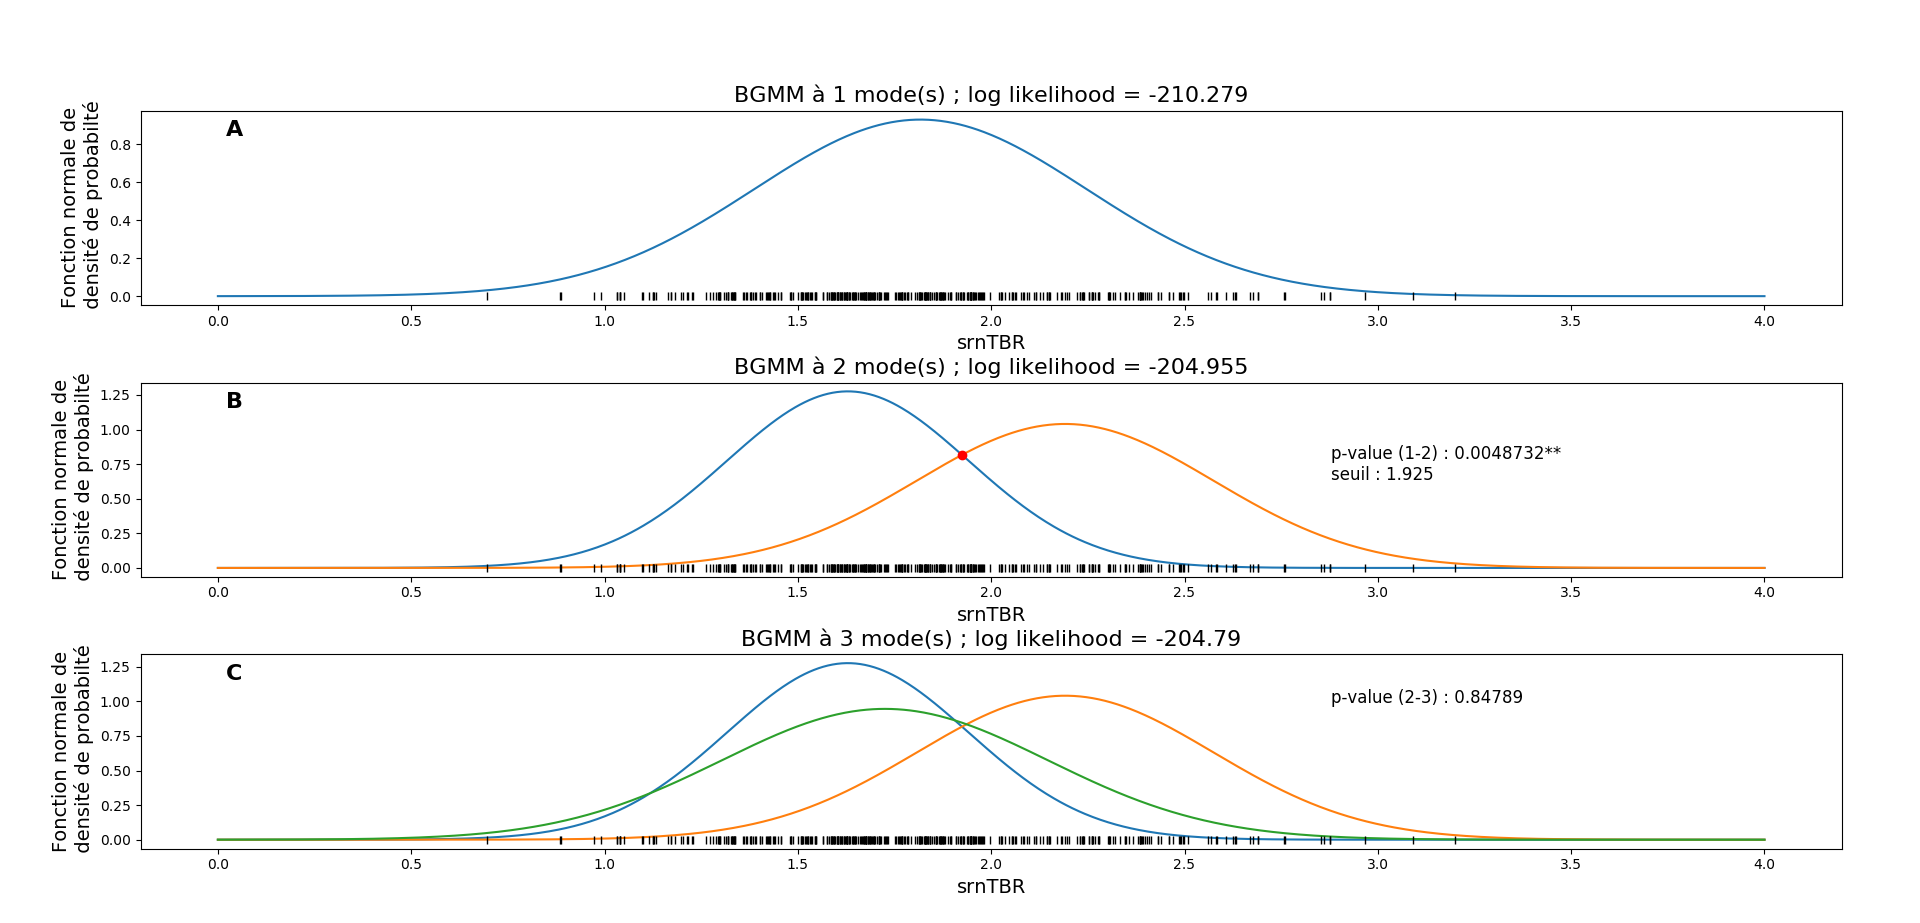
\includegraphics[width=1.0\linewidth]{figures/chapter-4/tbr-bgmm} 
  \caption{Tracés des distributions de \gls{srntbr} (\textit{rug plot}) avec \textbf{A)} 1-mode, \textbf{B)} 2-modes et \textbf{C)} 3-modes du \gls{bgmm} superposés. P-value (1-2) correspond
	à la p-value du test de déviance comparant les \gls{bgmm} à 1 mode et 2 modes ; p-value (2-3) correspond à la p-value du test de déviance comparant les \gls{bgmm}
	à 2 modes et 3 modes. Significativité symbolisée par ** (seuil fixé à 0.01). Le seuil \gls{srntbr} est précisé pour le modèle à 2 composantes et représenté par un cercle rouge.}
  \label{Figure:tbr_bgmm} 
\end{figure}

Une différence statistiquement significative est observée dans la modélisation des distributions entre les modèles à 1 (modèle nul) et à 2 composantes 
du \gls{bgmm} (p-value = 0.005), alors qu'aucune différence statistiquement significative n'est observée entre les modèles à 2 (modèle nul) 
et à 3 composantes du \gls{bgmm} (p-value = 0.850). On peut donc en conclure que le \gls{bgmm} à 2 modes décrit mieux la donnée que les deux
autres modes. 

Le \gls{gmm} arrive à la même conclusion : la distribution des \gls{srntbr} semble bimodale (p-value pour la comparaison
entre le modèle à 1 mode (modèle nul) et à 2 modes = 0.002). Ainsi, les \textit{a priori} utilisés pour le \gls{bgmm} semblent bien 
représenter la donnée. 

\subsubsection{Méthode de Ward}
Tout d'abord, les résultats d'un partitionnement suivant la méthode de Ward sont représentés sur le dendrogramme présenté à la 
Figure~\ref{Figure:tbr_ward_dendrogram}. 

\begin{figure}[h!]
  \centering
	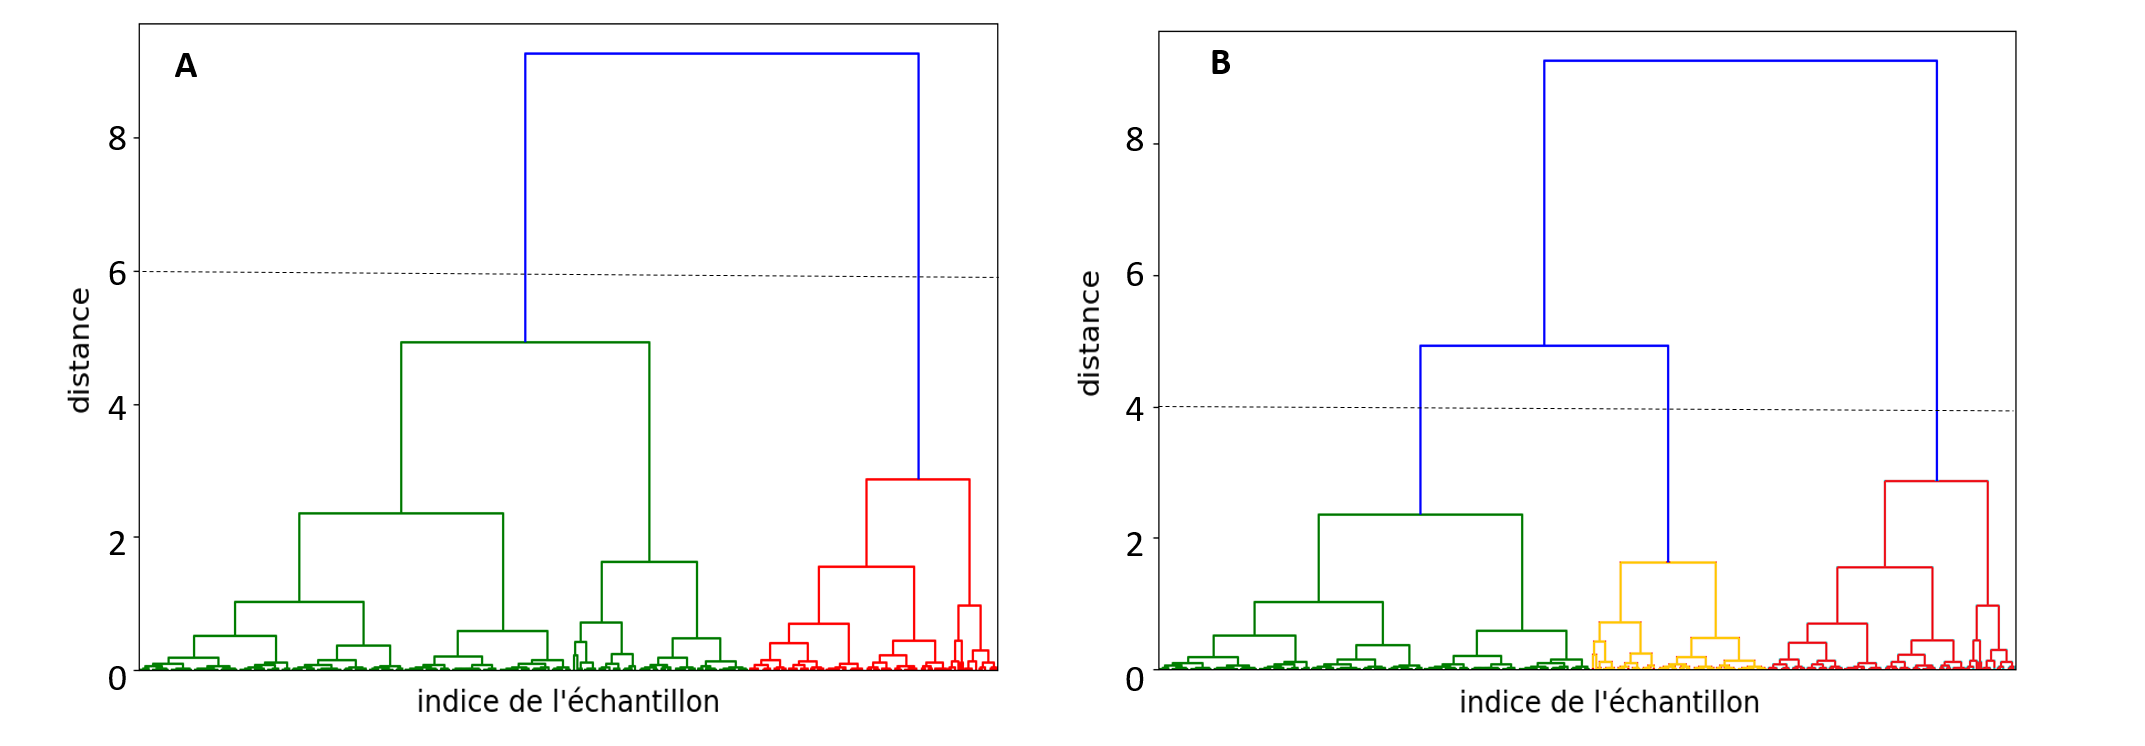
\includegraphics[width=0.5\linewidth]{figures/chapter-4/tbr-dendrogram-ward} 
  \caption{Dendrogramme représentant le partitionnement obtenu suivant la méthode de Ward. Tous les liens connectant des noeuds avec des distances plus 
	grandes ou égales à un seuil fixé à 6 sont colorés en bleu. Les deux clusters définis par les deux noeuds en dessous de ce seuil de 6 sont colorés différemment.}
  \label{Figure:tbr_ward_dendrogram}
\end{figure}

Cette représentation permet de supposer que les données pourraient être séparées en 2 \textit{clusters} (en rouge et vert) 
mais aussi en 3 (2 verts et 1 rouge). Les résultats d'un partitionnement en 2 et 3 \textit{clusters} sont représentés à la Figure~\ref{Figure:tbr_ward_histograms}.

\begin{figure}[h!]
  \centering
	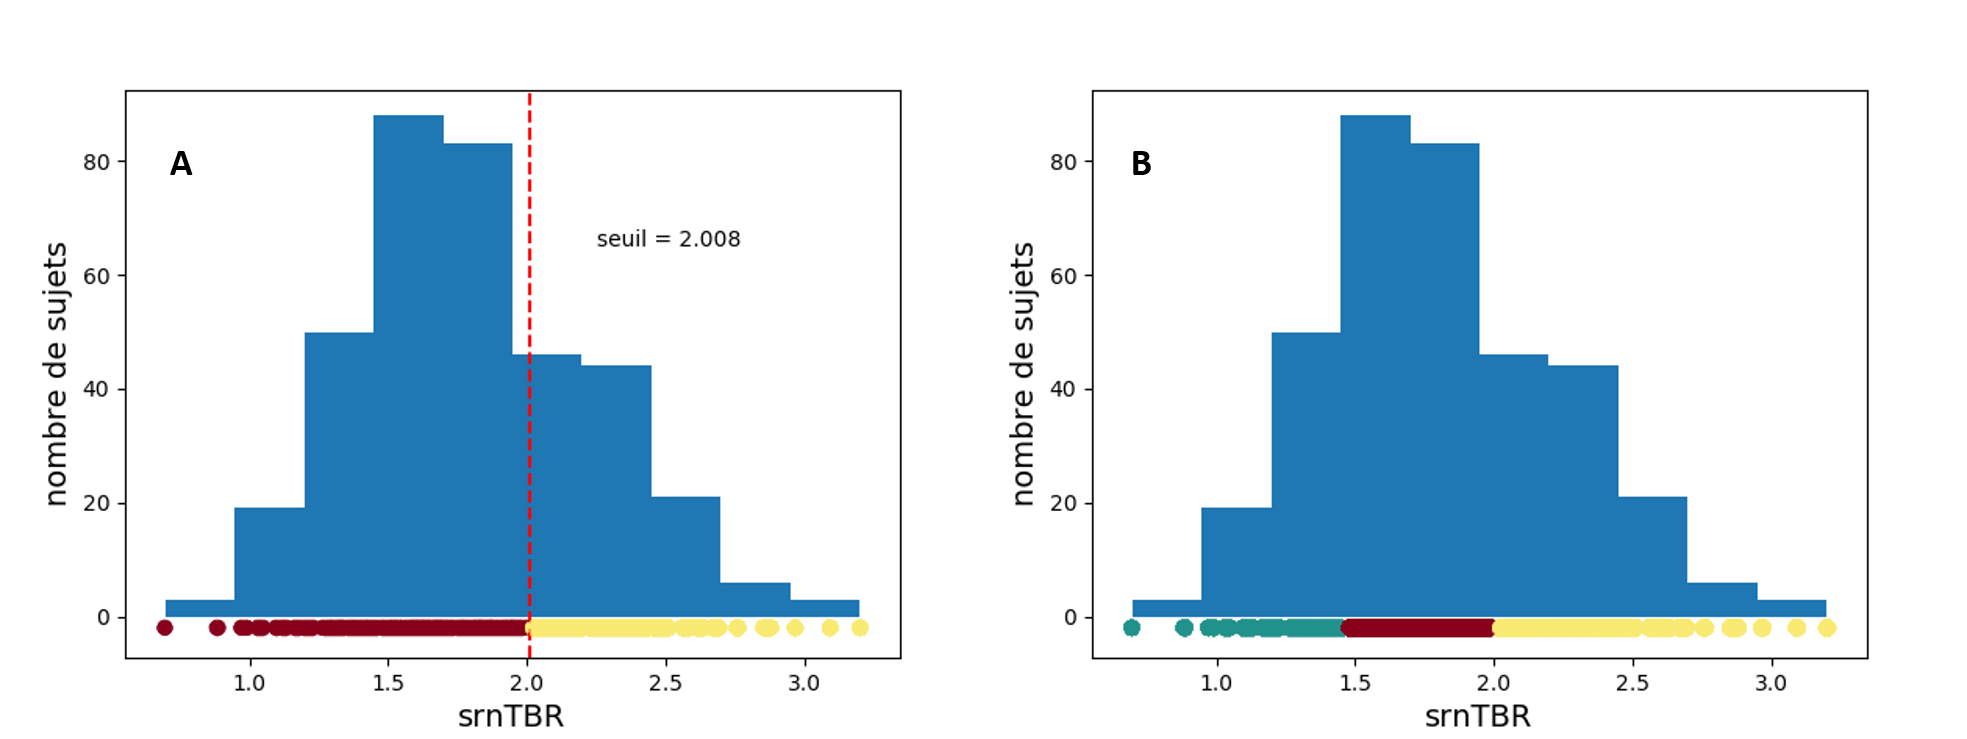
\includegraphics[width=1.0\linewidth]{figures/chapter-4/tbr-histogram-ward} 
  \caption{Distribution des \gls{srntbr} répartis en \textbf{A)} : 2 \textit{clusters} (rouge et jaune) et \textbf{B)} : 3 \textit{clusters} 
	(vert, rouge et jaune). Le seuil séparant la distribution des \gls{srntbr} en deux groupes est représenté par la ligne verticale en pointilés rouges sur la 
	figure \textbf{A}.}
  \label{Figure:tbr_ward_histograms}
\end{figure}

Dans le cas du partitionnement en 3 groupes, le groupe des \gls{srntbr} élevés est toujours identifié (en jaune), le troisième groupe est formé dans 
la sous population des \gls{srntbr} plus faibles. 

\subsubsection{DBSCAN}

Les paramètres $MinPts$ et $\epsilon$ de l'algorithme \gls{dbscan} sont tout d'abord calculés. Etant donné qu'ici $MinPts = $ 6, 
l'algorithme des \gls{knn} prend k = 6, on obtient alors le grahique des distances k présenté à la Figure~\ref{Figure:tbr_dbscan_kdistance_plot}, 
où un coude est observé à $y$ = 0.048, valeur choisie pour $\epsilon$.

\begin{figure}[h!]
  \centering
	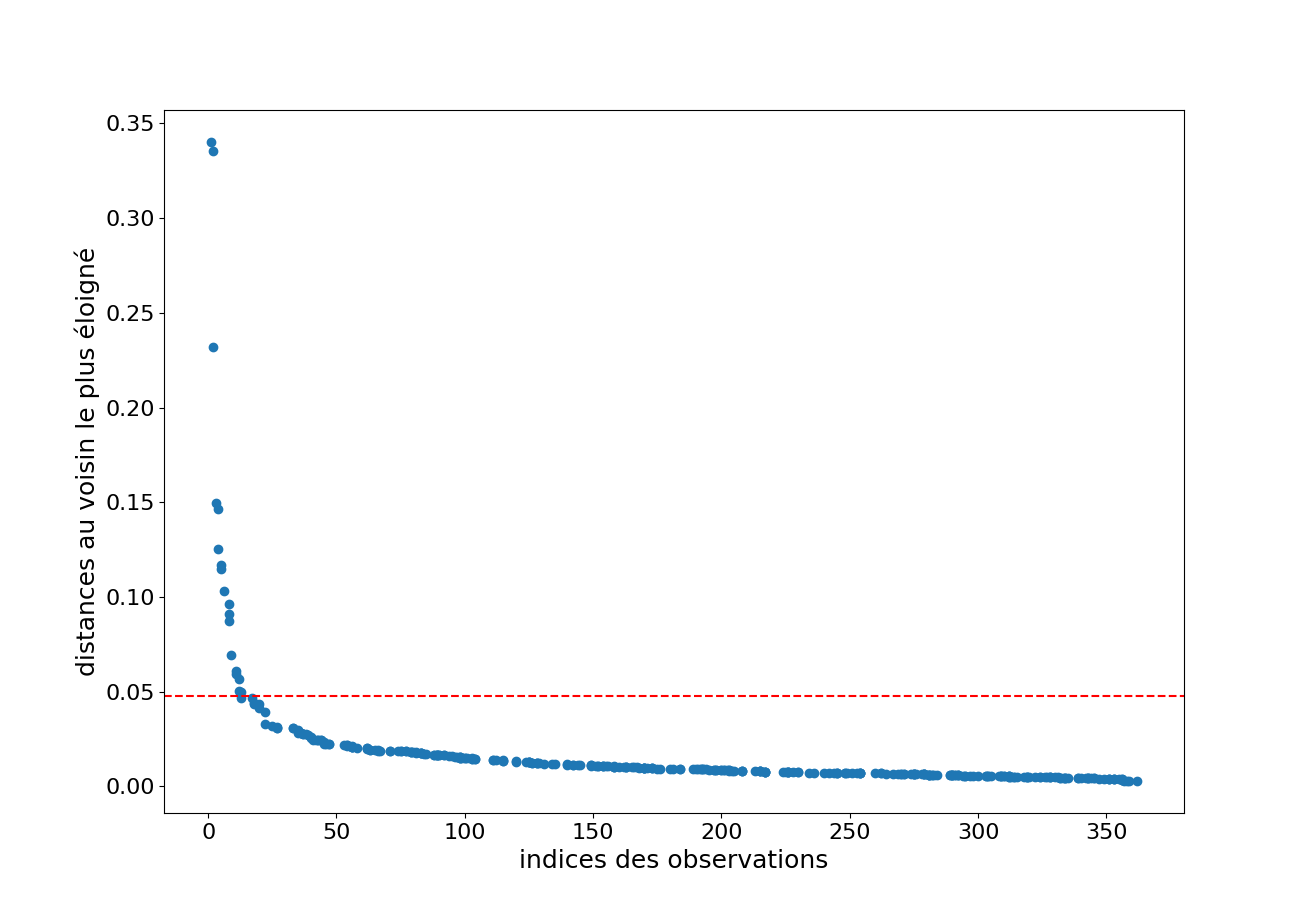
\includegraphics[width=0.7\linewidth]{figures/chapter-4/tbr-dbscan-knn-plot} 
  \caption{Graphique des k distances. La ligne en pointillés noirs coupe la courbe où le coude est identifié.}
  \label{Figure:tbr_dbscan_kdistance_plot}
\end{figure}

Le partitionnement par \gls{dbscan} est représenté à Figure~\ref{Figure:tbr_dbscan_clustering_plot} : deux groupes (en rouge et jaune) et 13 
points considérés comme du bruit et donc attribués à aucun groupe (en noir) sont identifiés. Le \textit{silhouette coefficient} de 0.388 
indique un partionnement convenable mais dont les groupes sont proches l'un de l'autre. 

\begin{figure}[h!]
  \centering
	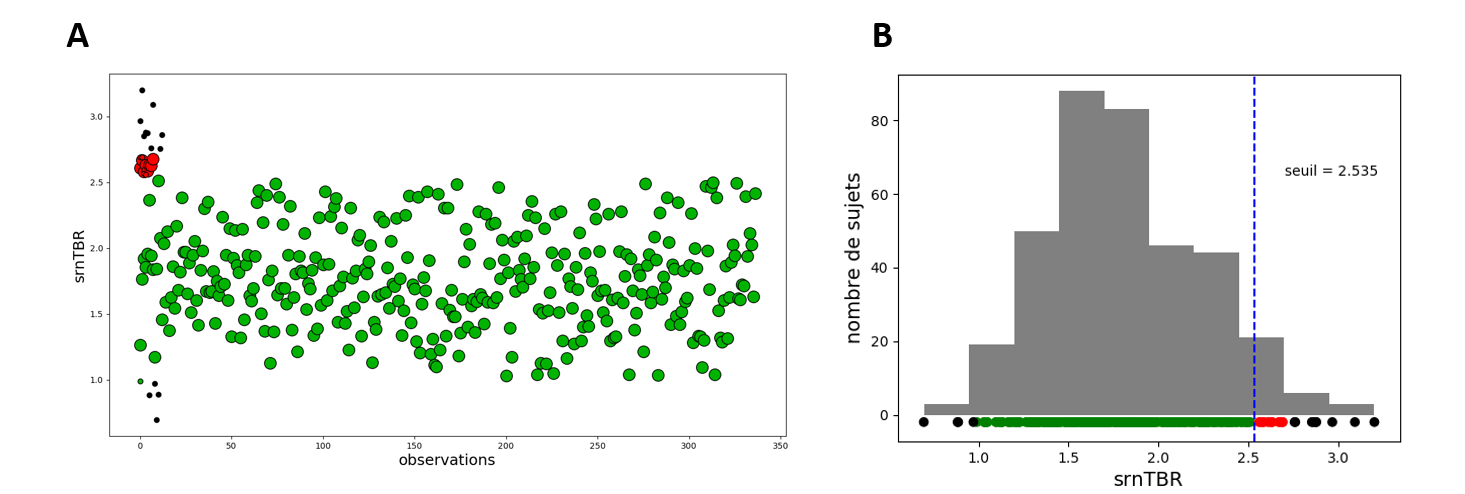
\includegraphics[width=1.0\linewidth]{figures/chapter-4/tbr-dbscan-clustering-plot} 
  \caption{Partitionnement obtenu par \gls{dbscan}. Deux groupes sont identifiés (en jaune et rouge) et 13 points sont considérés comme du bruit (en noir).
	En \textbf{B)} le seuil \gls{srntbr} est représenté par la droite verticale en pointillés rouges.}
  \label{Figure:tbr_dbscan_clustering_plot}
\end{figure}

Le groupe de \gls{srntbr} élevés (en jaune) contient peu d'observations et est très dense : ces valeurs varient peu d'un sujet à l'autre.


\subsection{Seuils identifiés}
Etant donné que les méthodes utilisées ici concluent toutes qu'un partitionnement des \gls{srntbr} en deux groupes est pertinent, il est possible de s'intéresser
au seuil qui permet de discriminer les données. Ce seuil est calculé pour toutes les méthodes sur les valeurs de \gls{srntbr} : pour convertir le seuil sur 
les valeurs de \gls {tbr}, il suffit de calculer le carré du seuil \gls{srntbr}. Les valeurs de seuil présentées par la suite correspondent au seuil
sur les données \gls{tbr}.

Les seuils obtenus sont : 
\begin{description}
\item[pour le \gls{bgmm} : ] le seuil identifié est de 3.7, il est représenté par un point rouge à la Figure~\ref{Figure:tbr_bgmm},
\item[pour le \gls{gmm} : ] le seuil identifié est de 3.8, valeur très proche de celle du seuil déterminé par le \gls{bgmm},
\item[pour la méthode de Ward : ] le seuil identifié lorsque le nombre de \textit{clusters} est fixé à 2 est de 4.032, représenté
par une ligne verticale en pointillés rouges à la Figure~\ref{Figure:tbr_ward_histograms},
\item[pour le \gls{dbscan} : ] le seuil identifié est de 6.426, schématisé à la Figure~\ref{Figure:tbr_dbscan_clustering_plot} par une ligne
verticale en pointillés rouges. 
\end{description}

Le courbe \gls{roc} calculée sur le \gls{bgmm} à deux composantes ajustant les \gls{srntbr} est tracée à la Figure~\ref{Figure:tbr_roc} et 
présente une \gls{auc} de 0.872. Sur cette courbe sont ajoutés les seuils obtenus par les autres méthodes et l'\gls{acc} à laquelle ils conduisent. 
La valeur des seuils affichée correspond au seuil sur les valeurs \gls{tbr}. 

\begin{figure}[h!]
  \centering
	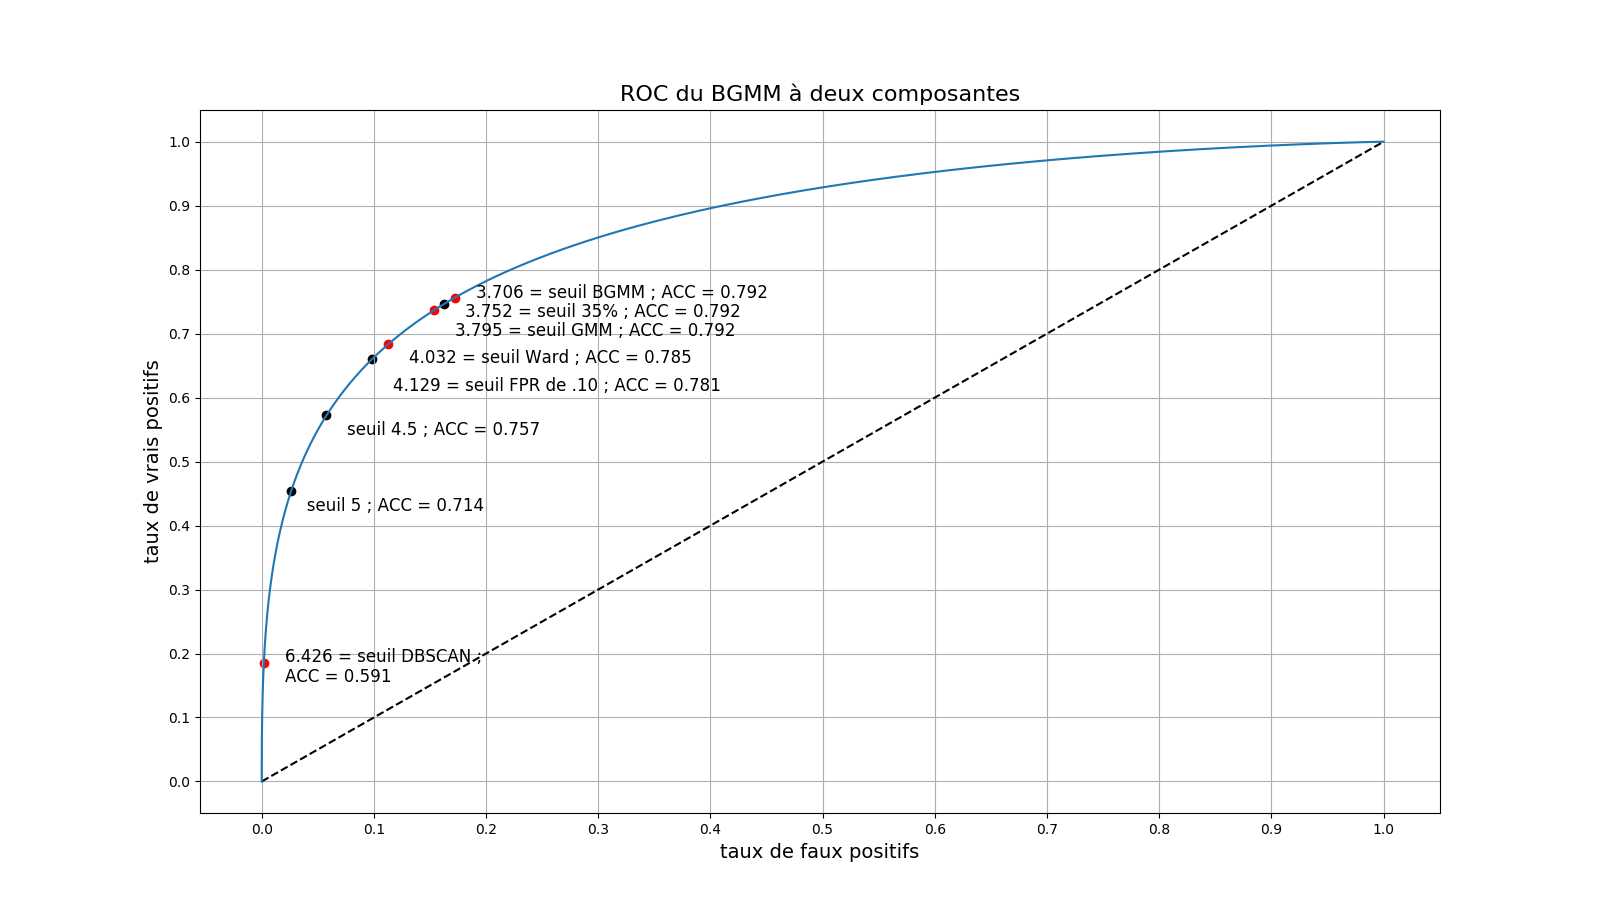
\includegraphics[width=1.0\linewidth]{figures/chapter-4/tbr-roc} 
  \caption{Courbe \gls{roc} obtenue avec le \gls{bgmm} à deux composantes (en bleu). Les seuils obtenus avec les méthodes implémentées ici sont représentés 
	par un point rouge sur la courbe ; les seuils issus de la littérrature sont représentés par un point noir. Pour chaque seuil la valeur de justesse (\gls{acc}) 
	est donnée.}
  \label{Figure:tbr_roc}
\end{figure}

Les seuils obtenus par les \gls{bgmm} et \gls{gmm} à deux modes et le seuil séparant 35\% de la population étudiée sont ceux conduisant à la plus grande \gls{acc} :
79.2 \%. Les deux seuils menant à des \gls{acc} bien plus faibles sont celui égal à 5 et celui trouvé par \gls{dbscan} avec respectivement une \gls{acc} de 71.4\%
et de 59.1\%. Toutefois, cette faible \gls{acc} est en partie compensée par un plus faible taux de faux positifs.

La Table~\ref{Table:tbr_thresholds_number_of_subjects} résume le nombre de sujets attribués au groupe \gls{tbr} élevés en discriminant les données 
avec les seuils présentés sur la courbe \gls{roc} à la Figure~\ref{Figure:tbr_roc}. La taille de ce groupe est assez stable, sauf pour le seuil identifié 
par \gls{dbscan} qui mène à un groupe comprenant seulement 5\% de la population étudiée.
\begin{table}[h!]
  \centering
  \caption{Poucentage de sujets considérés comme présentant un \gls{tbr} élevé pour chaque seuil étudié.}
  \fontsize{9}{11}\selectfont
\begin{tabular}{ ccc }
\toprule
Seuil \gls{tbr} utilisé & Valeur du seuil \gls{tbr} & \shortstack{Pourcentage d'observations \\ (sujets) au-dessus du seuil} \\
\midrule
\gls{bgmm} & 3.706 & 36\% \\
35\% & 3.752 & 35\% \\
\gls{gmm} & 3.795 & 33\%\\
Ward & 4.032 & 29\% \\
\gls{fpr} à 10\% & 4.129 & 28\% \\
4.5 & 4.5 & 24\% \\
5 & 5 & 19\% \\
\gls{dbscan} & 6.426 & 5.79\%\\
\bottomrule
\end{tabular}
  \label{Table:tbr_thresholds_number_of_subjects}
\end{table}


\section{Discussion}

Trois méthodes de partitionnement différentes ont été utilisées afin de déterminer si un groupe d'enfants avec un \gls{tbr} élevé existe et, auquel cas, 
le seuil à partir duquel le \gls{tbr} est considéré comme élevé est calculé. Ces résultats sont discutés ici puis les limites de cette analyse sont 
explorées.

\subsection{Groupes et seuils identifiés}

\subsubsection{Groupes d'enfants \gls{tdah}}

Le partitionnement par \gls{bgmm} montre que le modèle à deux composantes ajuste la distribution des \gls{srntbr} significativement mieux que le modèle
à une composante (p-value = 0.005). En ce qui concerne la comparaison entre le modèle à 2 composantes et celui à 3 composantes, même si ce dernier présente 
une \textit{log likelihood} un peu plus élevée (-204.790 contre -204.955), il n'y a pas de différence statistiquement significative entre ces deux modèles (p-value
= 0.850). Ainsi, en accord avec le rasoir d'Occam, le modèle le plus simple qui ajuste le mieux la donnée est retenu. Il est important de souligner
qu'ajouter des composantes au modèle va dans la plupart des cas augmenter la \textit{log likelihood}, c'est pourquoi, on s'intéresse à 
la significativité de cette augmentation pour éviter l'\textit{overfitting}. Le modèle \gls{bgmm} à deux composantes décrit donc le mieux la distribution
des valeurs de \gls{tbr}, ce qui indique qu'il existerait deux groupes distincts d'enfants \gls{tdah}, dont un présentant un \gls{tbr} élevé.

Cette conclusion obtenue avec le partitionnement par \gls{bgmm} est confirmée par les résultats du \gls{gmm} qui, par ailleurs, valident le choix de 
l'\textit{a priori} du \gls{bgmm}. 

L'\textit{agglomerative clustering} basé sur la distance de Ward montre que l'ensemble des données peut être réparti 
en deux ou trois groupes. Lors du partitionnement en deux groupes, un \textit{cluster} correspondant aux \gls{tbr} élevés et comprenant 29\% de la donnée
est identifié. Ce \textit{cluster} est toujours identifié lorsque le partionnement se fait en trois groupes : le nouveau groupe est formé dans la sous-population
des \gls{tbr} plus faibles. La méthode de Ward a déjà été utilisée lors de recherches 
précédentes sur l'identification de sous groupes chez les enfants \gls{tdah} basée sur l'\gls{eeg} \citep{Clarke2011}. 

L'algorithme \gls{dbscan} conduit également à deux \textit{clusters}, dont l'un correspond aux \gls{tbr} élevés avec un \textit{silhouette score} de 0.388 
qui permet d'être assez confiant dans le partitionnement retourné. Parmi les 13 points attribués à 
aucune classe, 9 correspondent à des sujets ayant un \gls{tbr} élevé. La possibilité qu'a cet algorithme de considérer certains points comme bruités, conduit à
une classe de \gls{tbr} élevés très dense. 

Par conséquent ces deux dernières méthodes confirment les résultats du \gls{bgmm} quant à l'existence d'un groupe de \gls{tbr} élevés, ce qui permet 
d'apporter de nouvelles preuves à l'hétérogénéité du \gls{tdah} déjà évoquée dans la littérature \citep{Arns2008, Arns2012, Barry2003, Clarke2011, 
Liechti2013, Loo2013, Loo2018}.

\subsubsection{Seuils de partitionnements}

Etant donné que le \gls{tdah} est un trouble hétérogène, tous les enfants \gls{tdah} ne vont pas nécessairement répondre au même traitement, ainsi le personnaliser 
pourrait être un moyen d'optimiser son efficacité pour chaque patient. L'existence de deux groupes distincts au sein de la 
population \gls{tdah} basée sur la valeur du \gls{tbr} étaye l'idée que le traitement par \gls{nfb} devrait être différent pour ces groupes. En effet, il semblerait
plus approprié que le protocole de diminution du \gls{tbr} ne soit proposé qu'aux enfants du groupe \gls{tbr} élevés et que les autres enfants entrainent un autre
neuromarqueur, comme par exemple le \gls{smr}. Ce modèle à deux protocoles a été notamment suggérés par \citet{Kerson2013, Arns2012} et a été évaluée lors 
d'un récent essai clinique (NCT02778360, Mensia Technologies, France, ClinicalTrials.gov, \citet{Bioulac2019}).

L'essai clinique de Mensia Technologies a fixé un seuil de \gls{tbr} = 4.5 qui permet d'assigner les sujets soit au groupe devant augmenter leur \gls{smr}, soit 
au groupe devant diminuer leur \gls{tbr}. La courbe \gls{roc} représentée à la Figure~\ref{Figure:tbr_roc}, montre que choisir un seuil \gls{tbr} égal à 4.5 conduit
à une \gls{acc} de 75.7\% et à un \gls{fpr} qui est environ deux fois plus faible que celui obtenu avec le seuil déterminé par le \gls{bgmm}. Toutefois, 
le \gls{tpr} est plus faible avec le seuil \gls{tbr} à 4.5. En supposant que le but du seuil est de maximiser l'\gls{acc}, le seuil \gls{bgmm} serait le 
plus adéquat, avec une \gls{acc} de 79.2\%.

Le seuil calculé à partir du \gls{bgmm} à deux composantes comduit à un groupe d'enfants au \gls{tbr} élevé représentant 36\% de la population étudiée. 
Ce pourcentage est en accord avec les précédentes études qui concluent qu'entre 25 et 40\% des patients \gls{tdah} présentent un \gls{tbr} élevé \citep{Arns2012}. 
De plus,\citep{Clarke2011} trouve que 35\% des patients \gls{tdah} ont un \gls{tbr} élevé. 
Les seuils identifiés par les méthodes utilisées ici permettent de former un groupe d'enfants \gls{tdah} présentant un \gls{tbr} élevé comprenant entre
25 et 40\% de la population totale, sauf dans le cas du \gls{dbscan} qui identifie un \textit{cluster}
de \gls{tbr} élevés comprenant seulement 5.79\% de la population. Ce faible pourcentage ainsi que la faible \gls{acc} obtenue laisse à penser
que la valeur de ce seuil ne sépare pas de manière fiable les deux groupes. Le seuil identifié par la méthode de Ward dans le cas de deux \textit{clusters}
est proche de celui trouvé par le \gls{bgmm} à deux composantes (4 contre 3.7), ce qui prouve une nouvelle fois qu'il existe un groupe d'enfants \gls{tdah}
présentant un \gls{tbr} élevé.

Au moment de choisir un seuil pour attribuer le protocole d'entrainement par \gls{nfb}, le seuil le plus précis n'est pas nécessairement le meilleur choix.
En effet, optimiser l'\gls{acc} revient à utilser le seuil du \gls{bgmm} de 3.7. Cependant, si on suppose que le protocole de diminution du \gls{tbr} est plus 
efficace pour les patients dans le groupe des \gls{tbr} élevés tandis que le protocole alternatif est efficace de la même façon pour tous les patients, il 
serait préférable de minimiser le \gls{fpr} plutôt que de maximiser l'\gls{acc}. Si on fixe raisonnablement un seuil menant à 10\% de \gls{fpr}, un seuil de 4.1
est obtenu, résultant en un \gls{tpr} de 67\% et une \gls{acc} de 78\%. Ainsi, nous recommandons l'utilisation d'un seuil \gls{tbr} de 4.1 pour attribuer
les protocoles d'entrainement du fait de son bon équilibre entre un faible \gls{fpr} et une \gls{acc} et un \gls{tpr} élevés. 
  
\subsection{Normalisation des Theta-Beta ratios}

Une des hypothèses posée pour avoir recours aux \gls{bgmm} et \gls{gmm} pour modéliser la distribution des \gls{tbr} est que ces derniers suivent une
distribution normale. En effet, un \gls{bgmm} appliqué à une distribution non normale identifierait de faux \textit{clusters} pour ajuster les données. 
Ainsi, pour être certain que l'hypothèse de normalité est valide, la distribution des \gls{tbr} de patients sains (provenant de la base de données \gls{cmi-hbn})
est analysée avec deux techniques de normalisation différentes : la \textit{log normalization} et la \textit{square-root-normalization}.

Les distributions de \gls{tbr} non normalisés, log normalisés et \textit{square-root} normalisés (les \gls{srntbr}) sont visuellement analysées à l'aide 
d'histogrammes, puis des tracés de probabilités (\textit{probability plots}) sont utilisés pour comparer ces distributions à des distributions normales 
et sont présentés à la Figure~\ref{Figure:tbr_normalization}. Le test de Shapiro-Wilk \citep{Shapiro1965} a été utilisé pour obtenir une mesure quantitative 
de la normalité des \gls{tbr} contrôles. Avec un seuil de significativité de 0.01, seule la distribution des \gls{srntbr} ne permet pas de rejeter l'hypothèse
nulle de normalité (p-value = 0.46). Ainsi, on suppose que les valeurs de \gls{srntbr} sont distribuées normalement. 

\begin{figure}[h!]
  \centering
	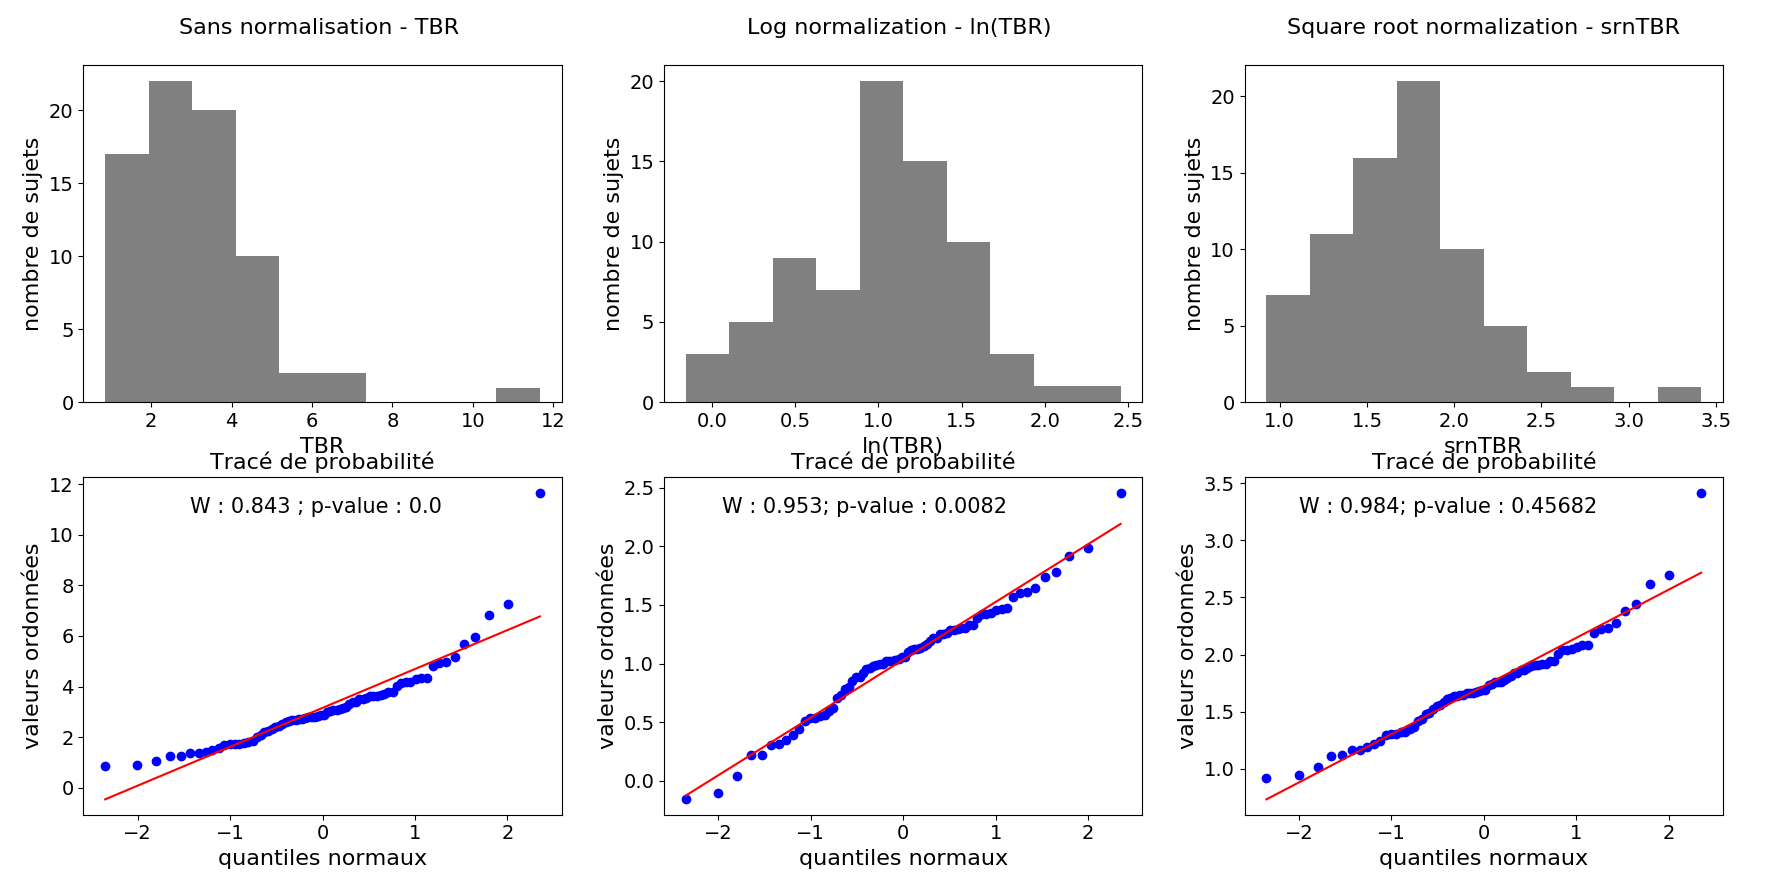
\includegraphics[width=1.0\linewidth]{figures/chapter-4/tbr-normalization} 
  \caption{Comparaison de techniques de normalisation des valeurs de \gls{tbr}. Les histogrammmes des distributions de valeurs \gls{tbr} non nomalisées,
	log normalisées et \textit{square-root} normalisées sont presentés à la première ligne. La seconde ligne contient les tracés de probabilités comparant les
	dstributions. La statistique W du test de Shapiro-Wilk et la p-value correspondante sont affichées sur chaque tracé de probabilité.}
  \label{Figure:tbr_normalization}
\end{figure}

\subsection{Calcul des Theta-Beta ratios}

La façon dont est calculé le \gls{tbr} est très variable dans la littérature, ce qui conduit à des valeurs variant entre 2 et 8 pour les sujets contrôles \citep{Arns2012,
Schutte2017}. La largeur de cet intervalle s'explique en partie par les diverses défintions du \gls{tbr}. En effet, le \gls{tbr} peut faire référence au ratio
des puissances ($\mu$V$^2$), des densités de puissance ($\mu$V$^2$/Hz), des voltages ($\mu$V) ou des densités de tensions ($\mu$V/Hz). 

Par ailleurs, la défintion des bandes de fréquences pour calculer le \gls{tbr} peuvent aussi varier : par exemple, le \gls{tbr} peut être obtenu à partir
de bandes de fréquence standards ou personnalisées grâce à l'\gls{iapf} du sujet. Ainsi, pour pouvoir comparer les valeurs de \gls{tbr} provenant de différentes
études, une définition homogène doit être mise en place. A travers cette analyse, nous recommandons de définir le \gls{tbr} de la façon suivante : 
le ratio entre la puissance dans la bande theta et la puissance dans la bande beta, avec une bande theta correspondant à [\gls{iapf} - 5Hz ; \gls{iapf} - 1Hz]
et une bande beta à [\gls{iapf} + 3Hz ; \gls{iapf} + 12Hz].

Il est important de souligner que les résultats de cette étude sont comparés à ceux où les \gls{tbr} sont calculés à partir de bandes de fréquence standards
les yeux fermés \citep{Zhang2017, Clarke2011}. Ces valeurs de \gls{tbr} sont donc différentes, mais nous supposons que les tendances dans la distribution et le
partitionnement obtenues ici doivent y être observées.

\subsection{Analyse des facteurs de confusion}

Les conclusions de cette analyse de la distribution des \gls{tbr} au sein de la population d'enfants \gls{tdah} doivent prendre en compte ses limitations.
En effet, deux points ont été approfondis ici pour juger de leur impact sur les résultats.

\subsubsection{Correction des artefacts oculaires}

La première source d'erreur possible de cette analyse est que les artefacts oculaires n'ont pas été corrigés sur les signaux \gls{eeg}. Ces artefacts
peuvent affecter les calculs de puissance et donc par ricochet les valeurs de \gls{tbr}. Les distributions des valeurs de \gls{tbr} sans et avec 
la correction d'artefacts oculaires basée sur la séparation aveugle de sources (\textit{blind source separation} en anglais) \citep{Barthelemy2017} 
ont été tracées à la Figure~\ref{Figure:tbr_eye_artifact_correction} où aucune grande différence entre les deux distributions n'est observée.
Par conséquent la correction des artefacts oculares ne semble pas influencer les valeurs de \gls{tbr} calculées.

\begin{figure}[h!]
  \centering
	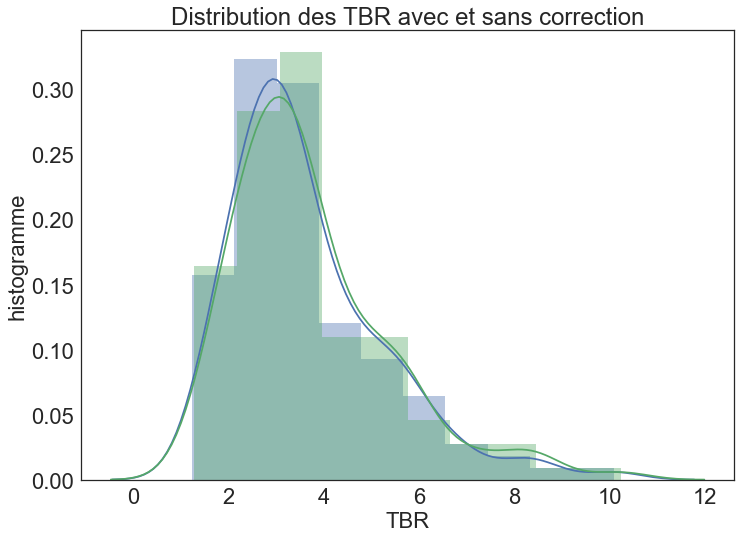
\includegraphics[width=0.5\linewidth]{figures/chapter-4/tbr-eye-artifact-correction} 
  \caption{Comparaison des distributions normalisées de \gls{tbr} calculés après correction des artefacts oculaires (en bleu) et sans correction (en vert).}
  \label{Figure:tbr_eye_artifact_correction}
\end{figure}

\subsubsection{Influence de l'âge}

Une autre source d'inexactitude pourrait être l'âge des sujets inclus dans l'analyse. En effet, la littérature a montré que les valeurs de \gls{tbr} varient
avec l'âge des enfants \citep{Liechti2013, Snyder2015, Perone2018}. De plus, le U-test de Mann-Whitney a été appliqué à nos données \gls{tbr} et a montré
qu'il existe une différence significative entre le groupe de \gls{tbr} faibles et de \gls{tbr} élevés définis avec le seuil de 3.7 du \gls{bgmm} à deux composantes
(p-value = 2.30e-15, U = 22 104, avec les âges médians $\pm$ l'ecart absolu médian de chaque groupe : 8.0$\pm$1.57 et 10.1$\pm$2.43). Par ailleurs, lorsqu'on trace
la distribution des âges dans chaque groupe représentée à la Figure~\ref{Figure:tbr_age_distribution}, on observe que plus les sujets sont âgés, plus leur 
\gls{tbr} semble faible.

\begin{figure}[h!]
  \centering
	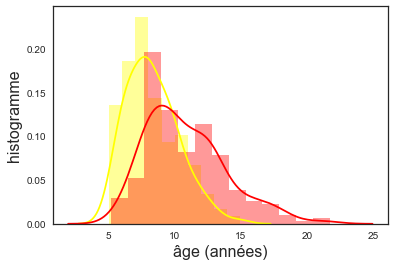
\includegraphics[width=0.5\linewidth]{figures/chapter-4/tbr-age-distribution} 
  \caption{Comparaison des distributions normalisées des âges dans les groupes de \gls{tbr} identifiés par le \gls{bgmm} à deux composantes.}
  \label{Figure:tbr_age_distribution}
\end{figure}

Ainsi, afin de prendre en compte cette relation, le \gls{bgmm} a été relancé une seconde fois sur un intervalle d'âges plus restreint : seuls les enfants
entre 7 et 13 ans sont inclus, ce qui correspond à un total de 560 sujets \gls{tdah} et de 53 sujets sains. les résultats obtenus sur cette nouvelle population 
conduisent à la même conclusion que sur l'intégralité de la population : deux groupes sont significativement identifiés (p-value entre le \gls{bgmm} à 1 et 2 
composantes = 2e-4) et un seuil \gls{tbr} de 3.84 est trouvé. 

Etant donné que les variations de \gls{tbr} sont censées augmenter avec l'âge, il serait intéressant d'effectuer cette analyse sur une sous population de jeunes (5 
à 6 ans) et plus grands (18 à 21) sujets. Cependant, faute d'un nombre suffisant d'informations dans ces extrêmes, cette étude ne peut pas être menée. Les prochaines
études sur le \gls{tbr} devront corriger les valeurs de \gls{tbr} de façon à ce qu'elles ne soient pas affectées par l'âge des patients.

\section{Conclusion}

Cette étude avait pour but d'explorer l'existence d'un groupe d'enfants \gls{tdah} basée sur leur \gls{tbr} extraits de signaux \gls{eeg} enregistrés les yeux 
ouverts. Les résultats montrent qu'il existerait deux groupes : un avec un \gls{tbr} élevé, et l'autre avec des valeurs de \gls{tbr} normales. Bien que les 
distributions de ces deux \textit{clusters} se superposent, le seuil de séparation le plus précis est de 3.7. La confirmation de l'existence de deux groupes
distincts est importante pour l'utilisation du \gls{nfb} pour traiter le \gls{tdah}. En effet, cela indique qu'un traitement par \gls{nfb} proposant deux protocoles
en fonction du \gls{tbr} pourrait être plus efficace que le même protocole de \gls{nfb} appliqué à tout le monde. A partir des résultats de cette étude, un seuil 
\gls{tbr} de 4.1 est recommandé pour assigner les protocoles de \gls{nfb}.